
\section{Cosmic antiprotons measurement}

%% First two antiproton experiments
Cosmic rays were discovered in 1912 \cite{NobelCosmicRay}, the antiproton was discovered in 1955 \cite{NobelAntiproton}, and the first measurements of cosmic antiproton component were performed in 1979 \cite{CosmicAntiprotonBogomolov1979, CosmicAntiprotonGolden1979}, when two pioneering balloon flight experiments published their results about cosmic antiprotons independently. The first one was carried out by Bogomolov et al. and the data taking was from 1972 to 1977 by three individual flights, the residual air was 11 g/cm$^2$ so a correction was needed. The result showed two candidates of cosmic antiprotons in the kinetic energy range of 2-5 GeV. The second one was carried out by R. L. Golden et al. in Palestine in Texas and the data taking was from June 21 to June 22 1979. The residual air in the flight altitude was 5.4 g/cm$^2$. The spectrometer had a superconducting magnet and the group reported 46 antiproton candidates from 5.6 to 12.5 GV. 

% Comment out
\begin{comment}
%In figure \ref{First2PbarExp}, the cosmic antiproton candidates in those two experiments are shown.
\begin{figure}[h] \centering   
\subfigure[] { \label{}    
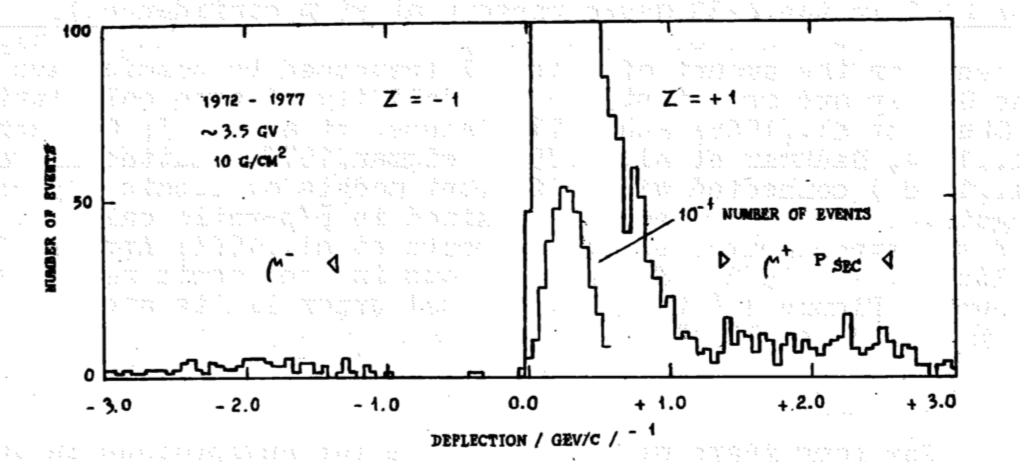
\includegraphics[width=0.45\textwidth, height=0.19\textheight]{Figures/chapter2/CosmicAntiprotonsMeasurement/Bogomolov1979.png} 
}    
\subfigure[] { \label{}    
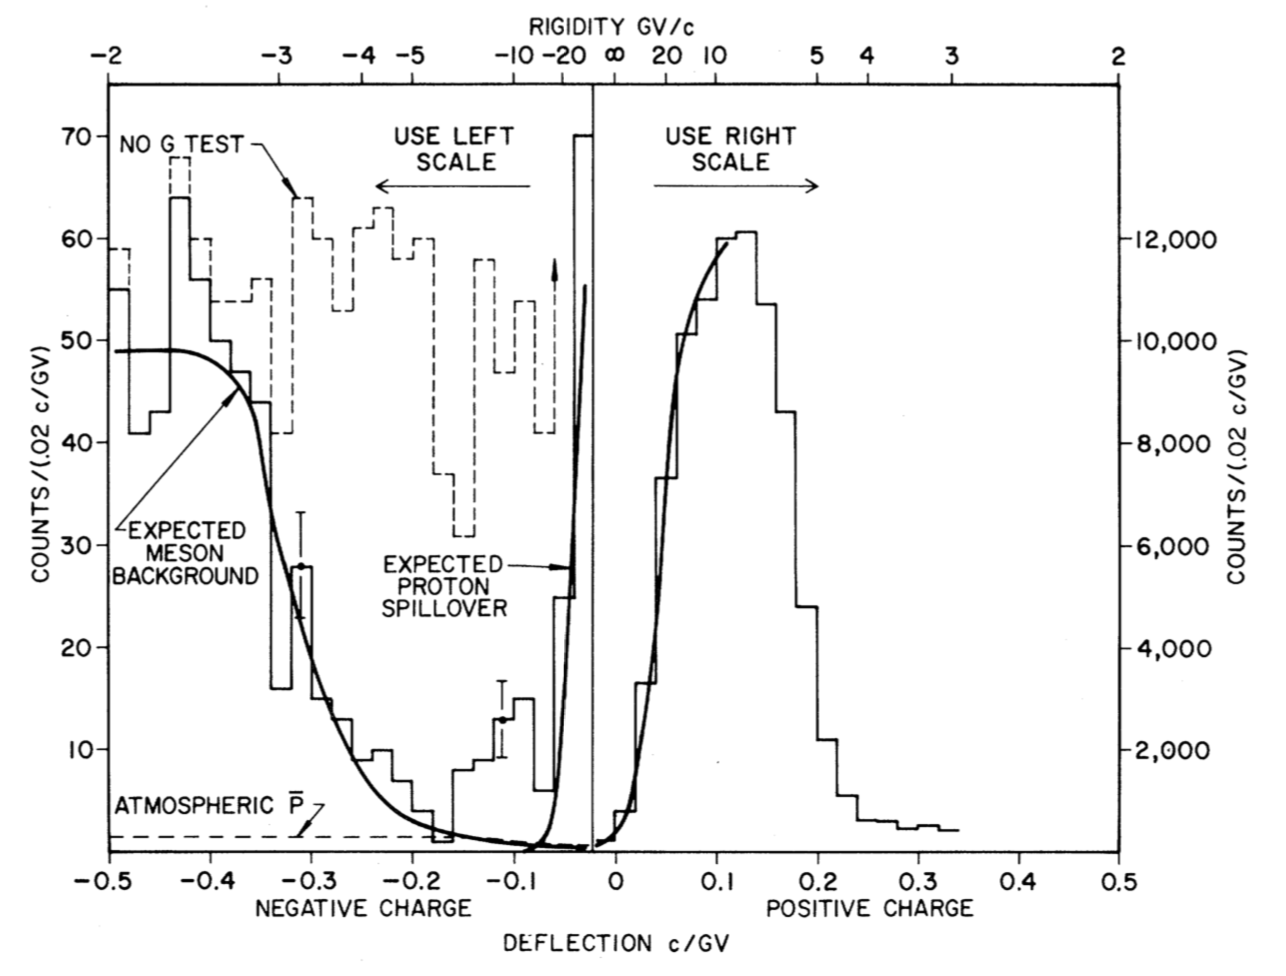
\includegraphics[width=0.45\textwidth, height=0.3\textheight]{Figures/chapter2/CosmicAntiprotonsMeasurement/Golden1979.png}    
}      
\caption{a). The antiproton signals in deflection (1/Rigidity) from the balloon flight experiment carried out by Bogomolov et al. in 1979 \cite{CosmicAntiprotonBogomolov1979}. b). The antiproton signals in deflection from the balloon flight experiment carried out by Golden et al. in 1979 \cite{CosmicAntiprotonGolden1979}}
\label{First2PbarExp}    
\end{figure}
\end{comment}

%% Bess and Pamela, AMS2016 Resul
% BESS 
After decades of effort, many cosmic ray experiments published results about cosmic antiprotons. For example, the BESS experiment, which is a balloon flight experiment \cite{BESSExperiment}, had nine successful flight campaigns since 1993. Then the apparatus was upgraded and renamed as BESS-Polar. The BESS-Polar was carried out in 2004 and 2008 respectively in the Antarctic \cite{BESSPolarExperiment1, BESSPolarExperiment2} and both flights measured the cosmic antiprotons \cite{BESSPolar1AntiprotonPaper, BESSPolar2AntiprotonPaper}. In the final result from the BESS-Polar II experiment, the group used data taken from Dec 2007 to Jan 2008 (a period corresponding to a  solar minimum) and reported the measurement of 7886 cosmic antiprotons in the kinetic energy range from 0.17 to 3.5 GeV \cite{BESSPolar2AntiprotonPaper}. 

% Comment out
\begin{comment}
Figure \ref{AntiprotoninBess2} shows the antiproton signals in $1 / \rm{\upbeta}$ versus Rigidity from BESS-Polar II.
\begin{figure}[h]
\centering
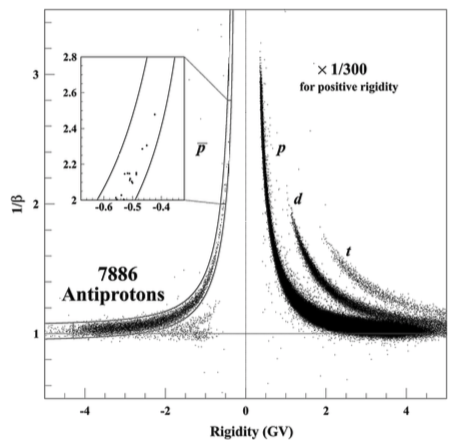
\includegraphics[width=0.5\textwidth, height=0.3\textheight]{Figures/chapter2/CosmicAntiprotonsMeasurement/AntiprotoninBess2.png}
\caption{The 7886 antiprotons signals and other components measured by BESS-Polar II in $1 / \upbeta$ versus Rigidity \cite{BESSPolar2AntiprotonPaper}.}
\label{AntiprotoninBess2}
\end{figure}
\end{comment}

%% Pamela and AMS2016
Due to the limited height of the balloon flight experiments, the correction of the residual air has to be considered to get a flux result above the atmosphere. The correction that the residual air creates can be overcome if a spectrometer is placed in space where the residual air is negligible. 

The first satellite-based cosmic antiproton measurement was performed by the PAMELA detector. PAMELA's mission lasted from June 2006 to February 2016 at a float altitude between 350 km and 610 km. The orbital period of the host satellite Resurs-DK1 was 94 min \cite{PamelaExperiment}. The PAMELA group published several antiproton results and the last one was in 2012 \cite{PamelaAntiproton100Paper, PamelaAntiproton180Paper, PamelaAntiproton350Paper} with a maximum measured energy of 350 GeV \cite{PamelaAntiproton350Paper}. This result shows a relatively flat antiproton to proton flux ratio in the high energy range, which is different from the traditional prediction of cosmic antiprotons from purely secondary production. In 2016 the AMS-02 experiment published its first result on cosmic antiprotons extending the measured rigidity range up to 450 GV using cosmic ray data collected during the first four years of its operation \cite{AMS02AntiprotonPRL2016}. The details of the AMS-02 experiment will be shown in the next chapter. \par

Apart from the experiment mentioned above, there are other balloon experiments that measured cosmic antiprotons. The antiproton flux results from these experiments are given in figure \ref{PbarFluxForDifferentExperiments}.  

\begin{figure}[h]
\centering
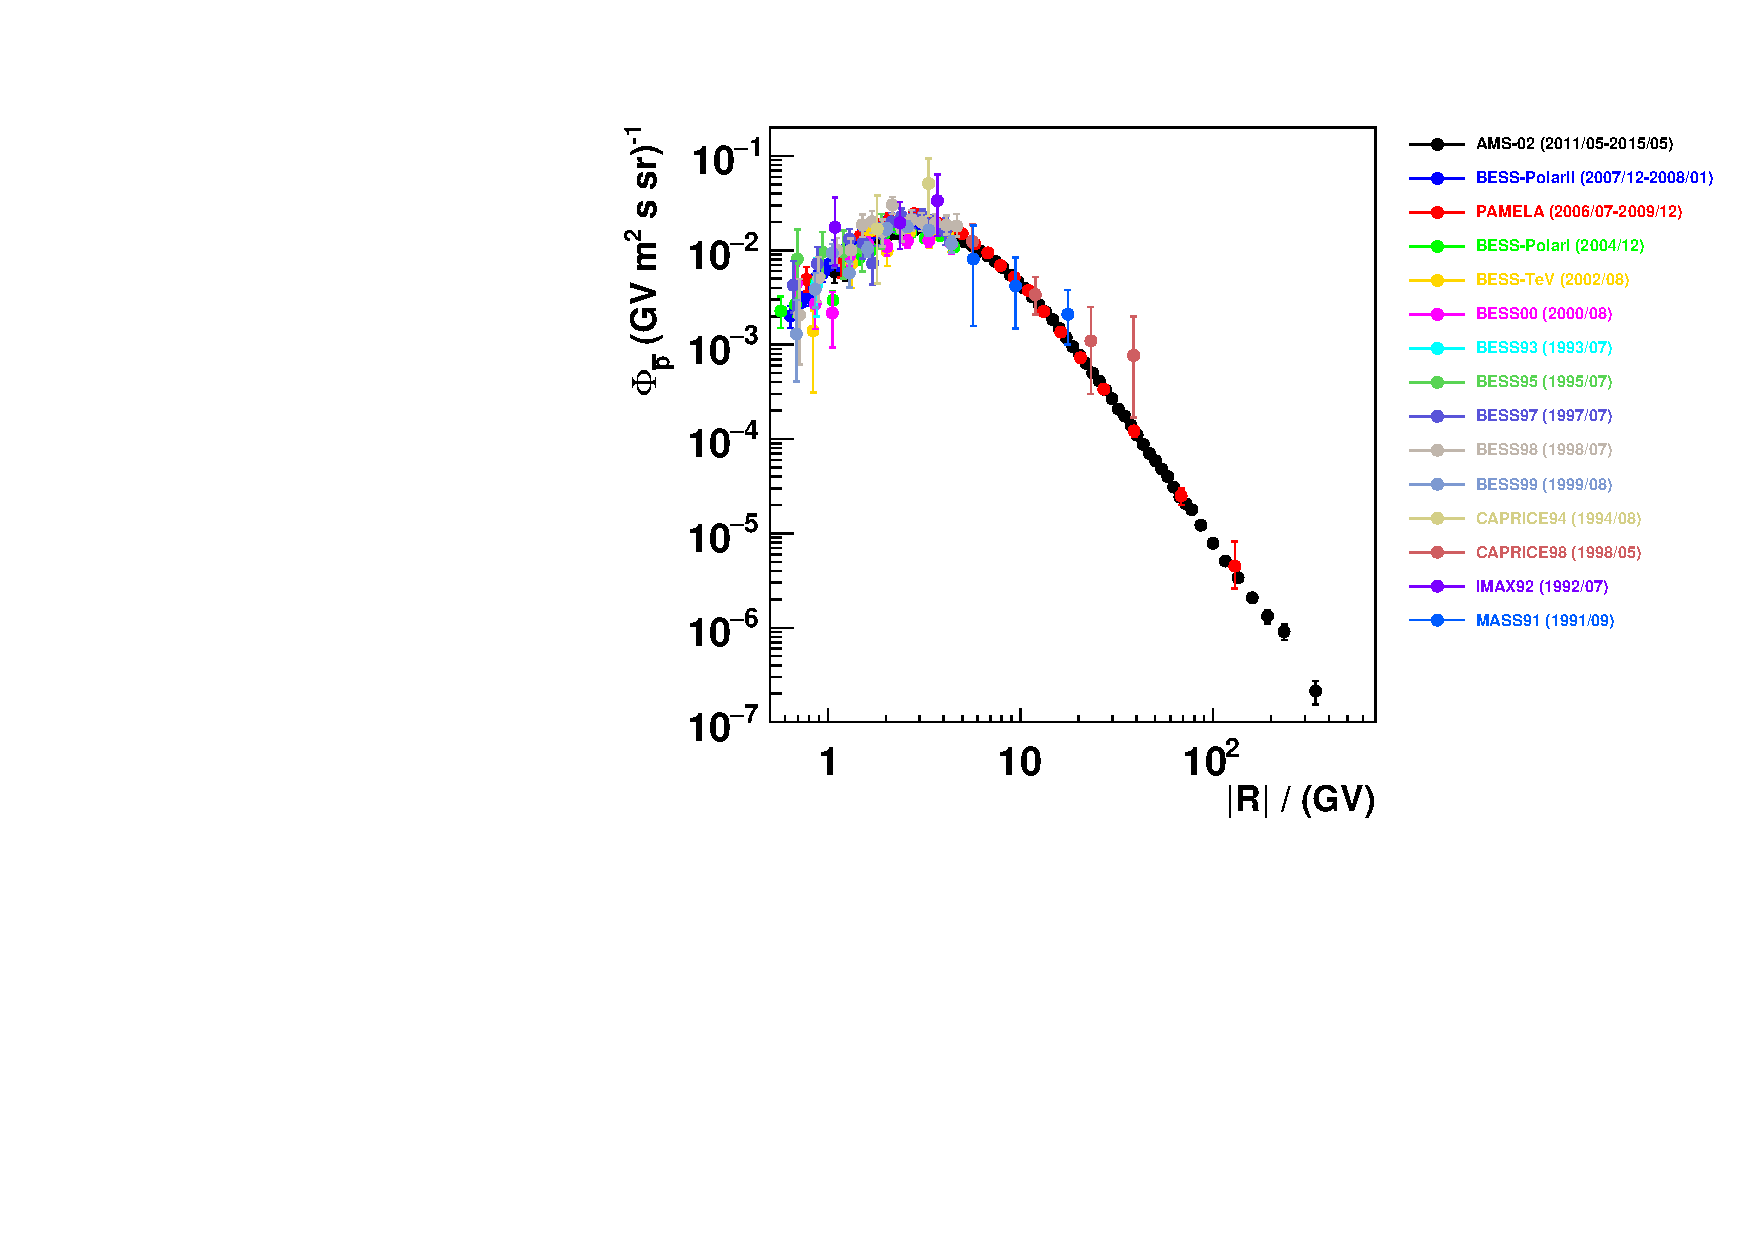
\includegraphics[width=1.0\textwidth, height=0.47\textheight]{Figures/chapter2/CosmicAntiprotonsMeasurement/PbarFluxForDifferentExperiments.pdf}
\caption[The measured antiproton flux.]{The antiproton flux measured by AMS-02 \cite{AMS02AntiprotonPRL2016}, BESS-Polar II \cite{BESSPolar2AntiprotonPaper}, PAMELA \cite{PamelaAntiproton350Paper}, Bess-Polar I \cite{BESSPolar1AntiprotonPaper}, Bess-TeV \cite{BESSTeV}, BESS00 \cite{BESS00and99}, BESS93 \cite{BESS93}, BESS95 \cite{BESS95}, BESS97 \cite{BESS97}, BESS98 \cite{BESS98}, BESS99 \cite{BESS00and99}, CAPRICE94 \cite{CAPRICE94}, CAPRICE98 \cite{CAPRICE98}, IMAX92 \cite{IMAX92}, MASS91 \cite{MASS91}. }
\label{PbarFluxForDifferentExperiments}
\end{figure}

% Pbar over P: 10^-4 so it's difficult.
Compared to antiproton measurement, the proton measurement is much easier since it is overwhelmingly dominant in cosmic rays. Many experiments have published the measurements of cosmic protons \cite{AMS02ProtonPaper, DAMPEProton2019, PAMELAProton2011, ATIC2Proton2009, CREAMIIIProton, NUCLEON-KLEMProton}. In this thesis, I will focus on the antiproton to proton flux ratio. Proton is primary cosmic ray and antiproton is believed to be secondary cosmic ray. Therefore, the antiproton to proton flux ratio is a probe to study the secondary to primary cosmic ray ratio, which can be used to investigate the source and the propagation of cosmic rays. Since the proton flux is about $10^4$ times greater than the antiproton flux, measuring the antiproton flux to 1\% accuracy requires a separation power of $\sim 10^6$. This leads to a challenge in high-energy measurement. 
   

